\documentclass[a4paper,12pt]{article}

%%% Работа с русским языком
\usepackage{cmap}					% поиск в PDF
\usepackage{mathtext} 				% русские буквы в формулах
\usepackage[T2A]{fontenc}			% кодировка
\usepackage[utf8]{inputenc}			% кодировка исходного текста
\usepackage[english,russian]{babel}	% локализация и переносы

%%% Дополнительная работа с математикой
\usepackage{amsmath,amsfonts,amssymb,amsthm,mathtools} % AMS
\usepackage{icomma} % "Умная" запятая: $0,2$ --- число, $0, 2$ --- перечисление

%% Номера формул
%\mathtoolsset{showonlyrefs=true} % Показывать номера только у тех формул, на которые есть \eqref{} в тексте.
%\usepackage{leqno} % Нумерация формул слева

%% Свои команды
\DeclareMathOperator{\sgn}{\mathop{sgn}}

%% Перенос знаков в формулах (по Львовскому)
\newcommand*{\hm}[1]{#1\nobreak\discretionary{}
{\hbox{$\mathsurround=0pt #1$}}{}}

%%% Работа с картинками
\usepackage{graphicx}  % Для вставки рисунков
\graphicspath{{Materials/graphics/}{images2/}}  % папки с картинками
\setlength\fboxsep{3pt} % Отступ рамки \fbox{} от рисунка
\setlength\fboxrule{1pt} % Толщина линий рамки \fbox{}
\usepackage{wrapfig} % Обтекание рисунков текстом

%%% Работа с таблицами
\usepackage{array,tabularx,tabulary,booktabs} % Дополнительная работа с таблицами
\usepackage{longtable}  % Длинные таблицы
\usepackage{multirow} % Слияние строк в таблице

%%% Теоремы
\theoremstyle{plain} % Это стиль по умолчанию, его можно не переопределять.
\newtheorem{theorem}{Теорема}[section]
\newtheorem{proposition}[theorem]{Утверждение}
 
\theoremstyle{definition} % "Определение"
\newtheorem{corollary}{Следствие}[theorem]
\newtheorem{problem}{Задача}[section]
 
\theoremstyle{remark} % "Примечание"
\newtheorem*{nonum}{Решение}

%%% Программирование
\usepackage{etoolbox} % логические операторы

%%% Страница
%\usepackage{extsizes} % Возможность сделать 14-й шрифт
\usepackage{geometry} % Простой способ задавать поля
	\geometry{top=25mm}
	\geometry{bottom=30mm}
	\geometry{left=25mm}
	\geometry{right=25mm}
 %

%%% Способ сделать тоже самое(но красивее:)
%\usepackage[margin=0.8in]{geometry}

 
\usepackage{fancyhdr} % Колонтитулы
 	\pagestyle{fancy}
 	\renewcommand{\headrulewidth}{0mm}  % Толщина линейки, отчеркивающей верхний колонтитул
 	\lfoot{}
 	\rfoot{}
 	\rhead{}
 	\chead{}
 	\lhead{ }
 	% \cfoot{Нижний в центре} % По умолчанию здесь номер страницы

\usepackage{setspace} % Интерлиньяж
%\onehalfspacing % Интерлиньяж 1.5
%\doublespacing % Интерлиньяж 2
%\singlespacing % Интерлиньяж 1

\usepackage{lastpage} % Узнать, сколько всего страниц в документе.

\usepackage{soulutf8} % Модификаторы начертания

\usepackage{hyperref}
\usepackage[usenames,dvipsnames,svgnames,table,rgb]{xcolor}
\hypersetup{				% Гиперссылки
    unicode=true,           % русские буквы в раздела PDF
    pdftitle={Заголовок},   % Заголовок
    pdfauthor={Автор},      % Автор
    pdfsubject={Тема},      % Тема
    pdfcreator={Создатель}, % Создатель
    pdfproducer={Производитель}, % Производитель
    pdfkeywords={keyword1} {key2} {key3}, % Ключевые слова
    colorlinks=true,       	% false: ссылки в рамках; true: цветные ссылки
    linkcolor=red,          % внутренние ссылки
    citecolor=green,        % на библиографию
    filecolor=magenta,      % на файлы
    urlcolor=blue           % на URL
}

%\renewcommand{\familydefault}{\sfdefault} % Начертание шрифта

\usepackage{multicol} % Несколько колонок

% Мои "дополнительные" пакеты
\usepackage{textcase} 
\usepackage{pdfpages}
\usepackage{amsmath}
\usepackage{titlesec}
\usepackage{floatrow}



\author{Подкидышев Алексей}
\title{Студент МФТИ ФИВТ - 1ый курс}
\date{\today}

%% Делаем красивый header:
\fancyhead[RO]{\footnotesize{\scshape\nouppercase{~\leftmark}}}
%% Делаем красивый header END

%Делаем большой отступ между section и subsection
\titlespacing*{\section} {0pt}{3.5ex plus 1ex minus .2ex}{2.7ex plus .2ex}
\titlespacing*{\subsection} {0pt}{2.7ex plus 1ex minus .2ex}{1ex plus .2ex}


\begin{document} % конец преамбулы, начало документа

\begin{center}
	\textit{\MakeTextUppercase{федеральное государственное автономное учреждение}}
		
	\vspace{0.5ex}
	
	\textbf{ \\ \MakeTextUppercase{<<Московский Физико-технический институт>>}}
\end{center}
\vspace{13ex}
\begin{flushright}
	\noindent
	{Александр Андреевич Харитонов,\\
	Подкидышев Алексей Сергеевич}
	\\
	\textit{Студенты факультета инноваций\\ и высоких технологий\\(группа 792)}
\end{flushright}
\begin{center}
	\vspace{23ex}
	\line(1,0){430}\\[4ex]
	{\LARGE\textbf{Лабораторная работа 1.3}}
	\vspace{2ex}
	
		
	\textbf{\large{<<Эффект Рамзауэра - рассеяние медленных электронов на атомах>>}}\\[3ex]
	\line(1,0){430}\\[5ex]
	\vfill
	Долгопрудный 
	
	{\today}
\end{center}

\newpage
\tableofcontents
\newpage
\renewcommand{\headrulewidth}{1pt}

\section{Описание работы}
%ссылка на таблицу: \url{https://docs.google.com/spreadsheets/d/1yUXbJdT5ChGKSeWxkUfRiLYM44lFkTVWOOHRGSaDYNM/edit#gid=0}\\
%ссылка на лабник: \url{https://mipt.ru/education/chair/physics/S_V/labs/1.3.pdf}

\subsection{Установка}
\indent В нашей работе для изучения эффекта Рамзауэера используется татрон, заполненный инертным газом. Схематическое изображение тратрона и его конструкция приведены на рис. 1.
\begin{wrapfigure}{r}{0.48 \textwidth}
    \vspace{-100pt}
    \begin{center}
        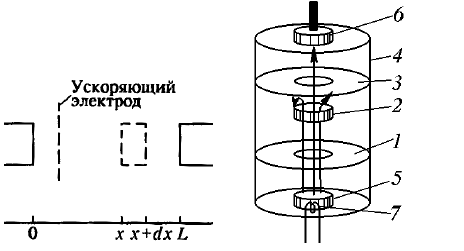
\includegraphics[width=0.89 \textwidth]{pic1.png}
    \end{center}
    \caption{Схема тиратрона (слева) и его конструкция (справа): 1, 2, 3 сетки, 4 внешней металлический цилиндр, 5 катод, 6 анод, 7 накаливаемая спираль}
\end{wrapfigure}
\indent Электроны, эмитируемые катодом тиратрона, ускоряется напряжением $V$, приложенным между катодом и ближайшей к нему сеткой. Затем электроны рассеиваются на атомах инертногояза. Все сетки 1,2,3 соединены между собой и имеют одинаовый оптенциал, примерно равный потенциалу анода 6. Поэтому между первой сеткой 1 и андом практические нет поля. 
\indent Рассеяные электроны отколняются в сторону и уходят на сетку, а оставшаяся часть электронов достигает анода и создаёт анодный ток $I_a$. Таким образом, поток электронов $N(x)$ на расстоянии $x$ от ускоряющей сетки уменьшается с ростом $x$ от начального значения $N_0$ у катода до нектороного значения $N_a$ у анода.
\subsection{Теоритическая часть}
\textbf{ВАХ тиратрона:} Выделим в газе на расстоянии $x$ тонкий слой с площадью поперчного сечения $S$ и толщиной $dx$. Этот слой содержит $\nu = n_a S dx$ атомов газа.\\
\indent Суммарная рассеивающая поверхность:$\Delta =\nu \cdot \Delta_a$, $\Delta_a$ - площадь поперчного сечения атома.\\
\indent Вероятность рассеяния электрона в слое:
\[- \dfrac{dN}{N(x)} = n_a \Delta_a \omega(V) dx.\]
Итоговое уравнение для ВАХ:
\[I_a = I_0 \cdot e^{- C \omega(V)}, C = Ln_a\Delta_a, \]
где $I_0 = eN_0$ ток катода, $I_a = eN_a$ анодный ток.

\begin{wrapfigure}{r}{0.35 \textwidth}
    \vspace{-100pt}
    \begin{center}
        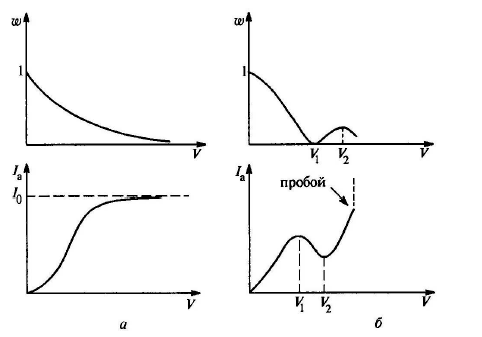
\includegraphics[width=0.9 \textwidth]{pic2.png}
    \end{center}
    \caption{Вероятность рассеяния электрона атомом инертного газа и ВАХ таратрона при классическом (а) и квантовом (б) рассмотрении}
\end{wrapfigure}
Согласно классическим представлениям, сечение рассеяния элетрона на атоме должно падать монотонно с ростом $V$ (обратно пропорционально квадратному корню из энергии
электрона), а значит ВАХ будет монотонно возрастающей функцией, как это показано на рис. 2а. По квантовым соображениям вероятность рассеяния электронов и соответствующая ВАХ должны иметь вид, показанный на рис. 2б.

По измеренной ВАХ тиратрона можно определить зависимость вероятности рассеяния электрона от его энергии из соотношения:
\[w(V) = -\frac{1}{C}\ln{\frac{I_a(V)}{I_0}}.\]

\begin{wrapfigure}{r}{0.48 \textwidth}
    \begin{center}
        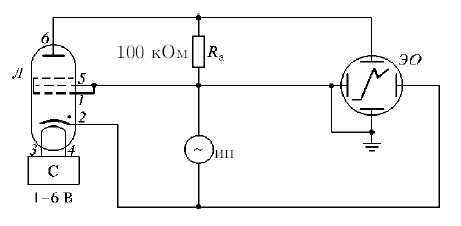
\includegraphics[width=0.89 \textwidth]{pic3.png}
    \end{center}
    \caption{Схема включения тиратрона}
\end{wrapfigure}
Схема для изучения эффекта Рамзауэра приведена на рисунке. На лампу Л подается синусоидальное напряжение частоты 50 Гц от источника питания ИП, С --- стабилизированный блок накала катода; исследуемый сигнал подается на электронный осциллограф (ЭО); цифрами обозначеный номера ножек лампы.

Реально на экране ЭО удается наблюдать лишь один (первый) миниум в сечении рассеяния электронов и следующий за ним максимум. Дело в том, что уже при $n = 2$ напряженность поля очень высока и происходит пробой тиратрона. 

Схема экспериментальной установки, изображенная на рис. 8 в нашей работе конструктивно осуществлена следющим образом. Лампа-тиратрон ТГ3001/1.3Б, заполненная инертным газом, расположена непосредственно на корпусе блока источника питания (БИП). Напряжение к электродам лампы подается от источников питания, находящихся в корпусе прибора. Регулировка напряжения и выбор режима работы установки производится при помощи ручек управления, выведенных на лицевую панель БИП (рис. 4).
\begin{figure}[h]
    \begin{center}
        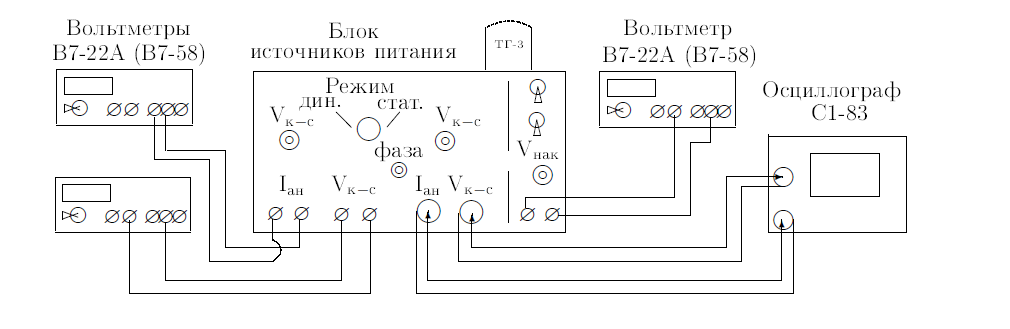
\includegraphics[width= \textwidth]{pic4.png}
    \end{center}
    \caption{Блок-схема экспериментальной установки}
\end{figure}
\newpage
\section{Ход работы}
\subsection{ВАХ тиратрона $I_a = f(U_c)$ на экране осциллографа С1-83}
\begin{enumerate}
    \item Поставим переключатель <<РЕЖИМ>> в положение <<ДИНАМИЧ>>.
    \item Установим напряжение накала лампы $V_{\text{накала}} = 2,95 \text{ В}.$
    \item Измерим на экране осциллографа напряжение между катодом и сеткой, соответствующее первому минимуму и максимуму на осциллограмме, при максимальном ускоряющем напряжении. Также оценим напряжение пробоя.
    \[\Delta V = 60 \text{мВ}, V_\text{пробоя} = 18\text{ В}.\]
    \item Чувствительность канала Х: $2 \text{ В/дел}.$
\begin{figure}[H]
    \begin{center}
        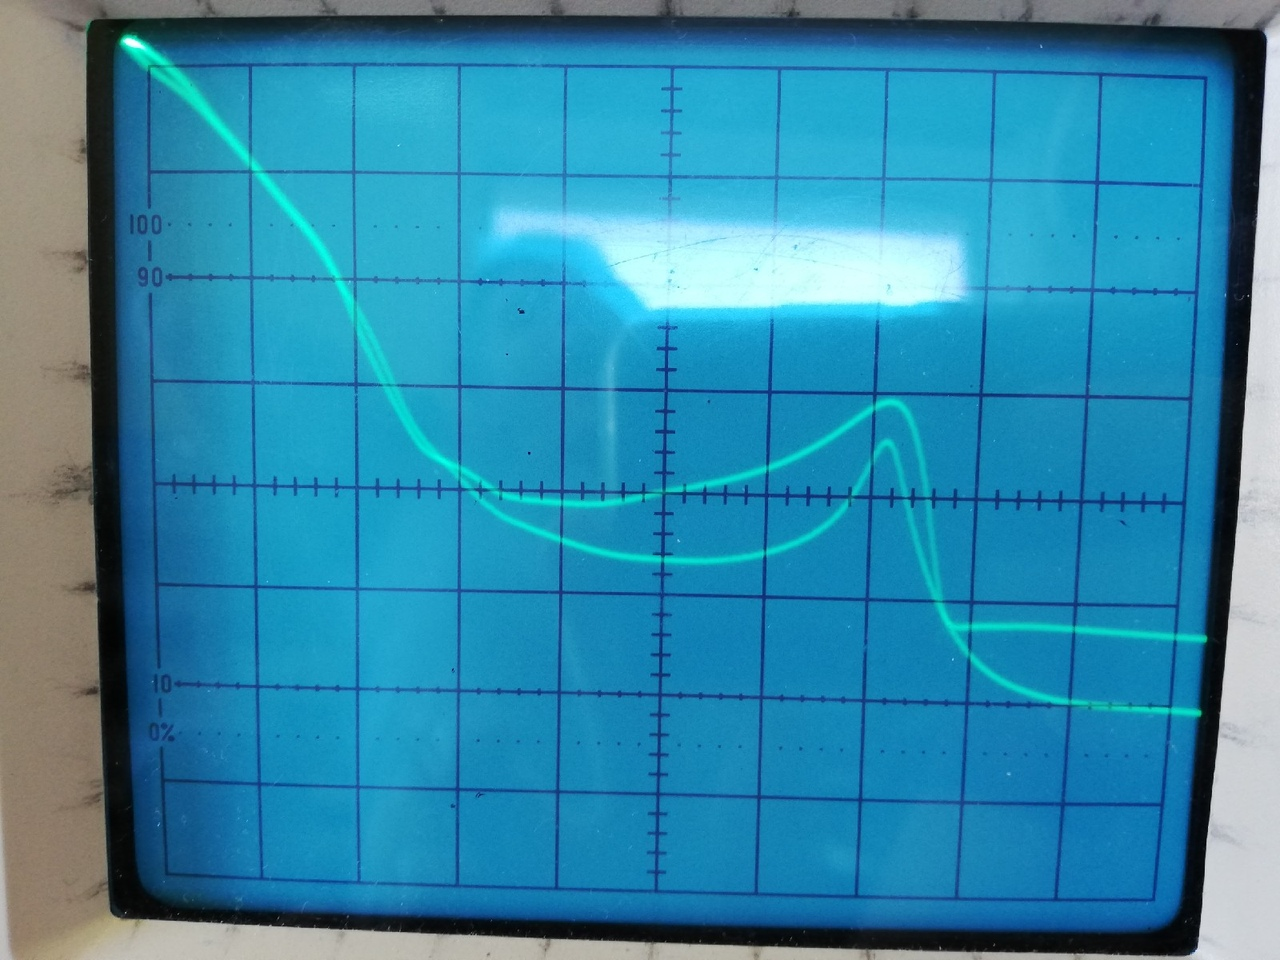
\includegraphics[width= 0.6 \textwidth]{oscilloscope1.jpg}
        \end{center}
    \caption{Осциллограмма при $V_\text{накала} = 2,95 \text{ В}$}
\end{figure}

    \item Повторим измерения при $V_\text{накала} = 2,56 \text{ В}:$ 
    \[\Delta V = 12 \text{ мВ}, V_{\text{пробоя}} = 20 \text{ В}.\]
    
\begin{figure}[H]
    \begin{center}
        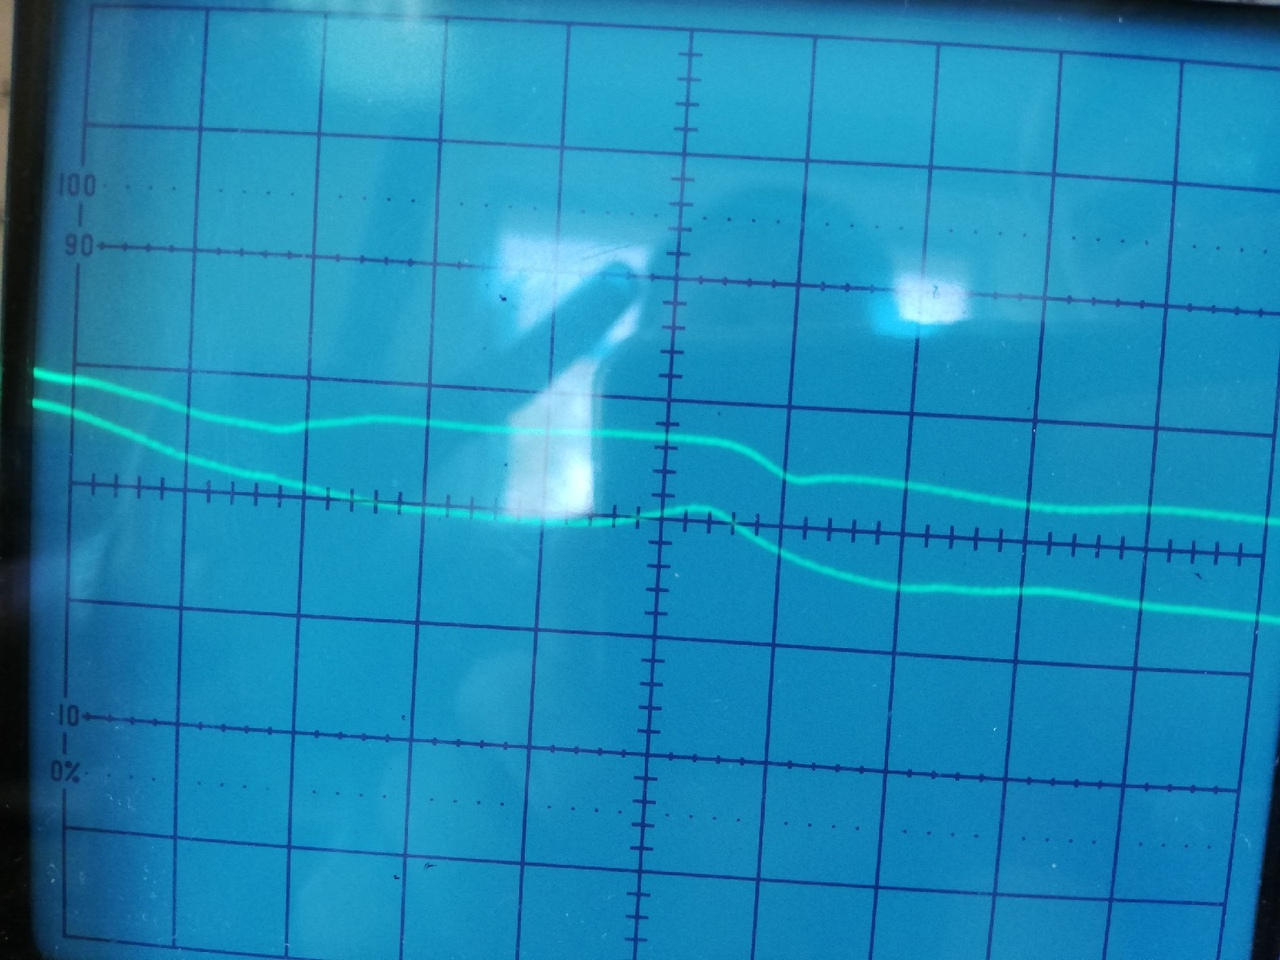
\includegraphics[width= 0.6 \textwidth]{oscilloscope2.jpg}
        \end{center}
    \caption{Осциллограмма при $V_\text{накала} = 2,56 \text{ В}$}
\end{figure}

Расчитаем размер электронной оболочки по формуле:
\[l = \frac{h\sqrt{5}}{\sqrt{32m(E_2-E_1)}}.\]
Получим $l = 2,8 \cdot 10^{-10} \text{ м}, \varepsilon_{l} = 7\%.$

\end{enumerate}

\newpage
\subsection{ВАХ в статическом режиме}
\begin{figure}[h]
\begin{floatrow}
	 \begin{tabular}{|l|l|}
\hline
\rowcolor[HTML]{FFECCB} 
\textbf{$V_\text{катода}$}  & \textbf{$I_\text{анода}, 10^{-6}$}    \\ \hline
1,50  & 0,10    \\ \hline
1,74 & 1,07 \\ \hline
1,98 & 4,07 \\ \hline
2,01 & 5,30  \\ \hline
2,20  & 7,46 \\ \hline
2,40  & 8,40  \\ \hline
2,64 & 7,82 \\ \hline
2,80  & 6,70  \\ \hline
3,08 & 5,58 \\ \hline
3,38 & 5,00 \\ \hline
3,78 & 4,42 \\ \hline
4,20  & 4,00 \\ \hline
4,74 & 3,75 \\ \hline
5,47 & 3,70  \\ \hline
6,34 & 3,60  \\ \hline
7,34 & 3,50  \\ \hline
8,20  & 3,53 \\ \hline
8,90  & 3,77 \\ \hline
9,70  & 3,93 \\ \hline
10,10 & 4,44 \\ \hline
\end{tabular}

\hspace{10ex}

\begin{tabular}{|l|l|}
\hline
\rowcolor[HTML]{FFECCB} 
\textbf{$V_\text{катода}$}  & \textbf{$I_\text{анода}, 10^{-6}$} \\ \hline
1,60  & 0,1 \\ \hline
1,83 & 1,09 \\ \hline
1,85 & 1,20 \\ \hline
2,03 & 2,70 \\ \hline
2,10  & 3,70 \\ \hline
2,24 & 3,78 \\ \hline
2,46 & 3,74 \\ \hline
2,64 & 3,30 \\ \hline
2,70  & 3,23 \\ \hline
2,92 & 2,80 \\ \hline
3,20  & 2,40 \\ \hline
3,50  & 2,06 \\ \hline
4,18 & 1,84 \\ \hline
4,54 & 1,74 \\ \hline
5,25 & 1,57 \\ \hline
6,10  & 1,45 \\ \hline
6,46 & 1,42 \\ \hline
7,37 & 1,35 \\ \hline
8,10  & 1,39 \\ \hline
9,60  & 1,54 \\ \hline
\end{tabular}

\caption{ВАХ в статическом режиме}
\end{floatrow}

\end{figure}

%график1:
\begin{figure}[h]
    \begin{center}
        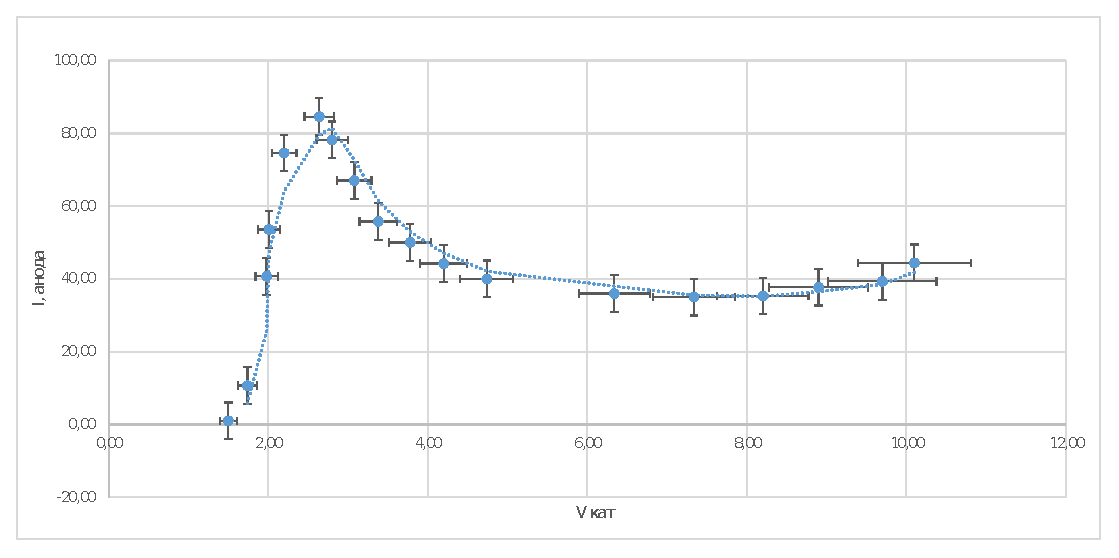
\includegraphics[width=1 \textwidth]{graph1.eps}
    \end{center}
    \caption{ВАХ в статическом режиме при $V_\text{накала} = 2,95 \text{ В}$}
\end{figure}

%график2: 
\begin{figure}[h]
    \begin{center}
        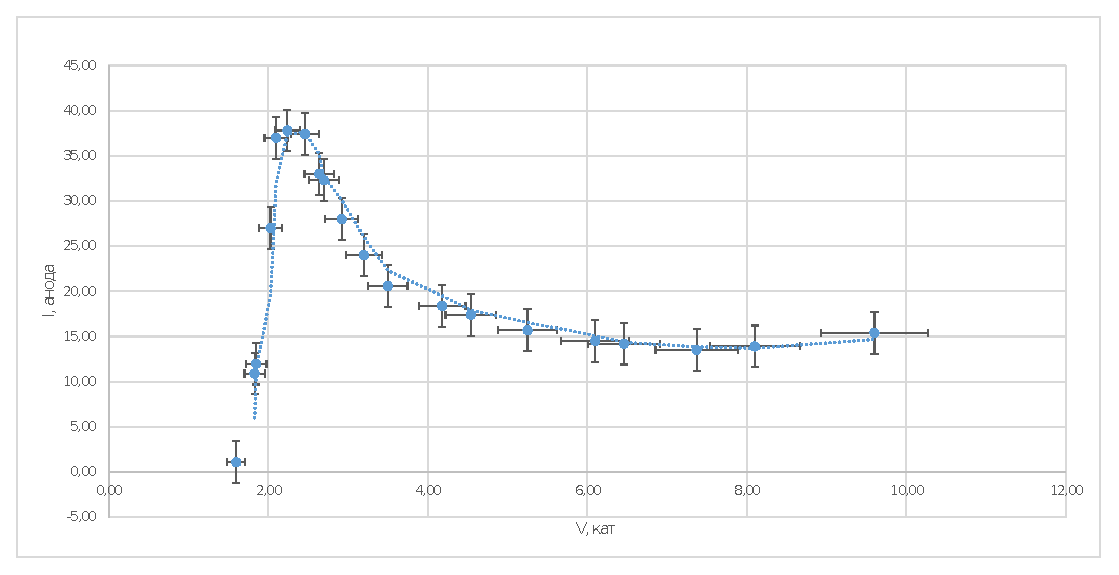
\includegraphics[width=1 \textwidth]{graph2.eps}
    \end{center}
    \caption{ВАХ в статическом режиме при $V_\text{накала} = 2,56 \text{ В}$}
\end{figure}

%Последние 2 графика, хз как их строить    
\begin{figure}[h]
    \begin{floatrow}
        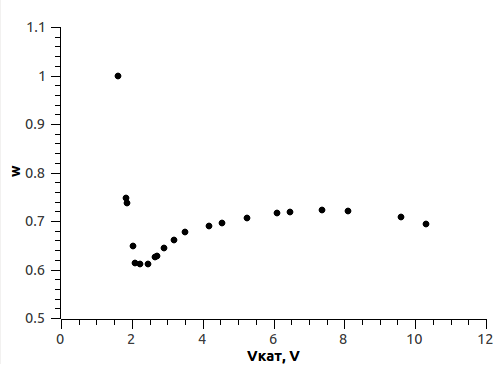
\includegraphics[width=0.5 \textwidth]{lol2.png}
        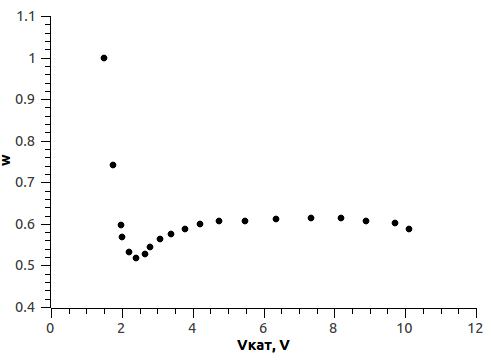
\includegraphics[width=0.5 \textwidth]{lol.png}
    \end{floatrow}
    \caption{Зависимости вероятности рассеяния электронов от энергии}
\end{figure}

\newpage

\begin{figure}[h]
    \begin{floatrow}
        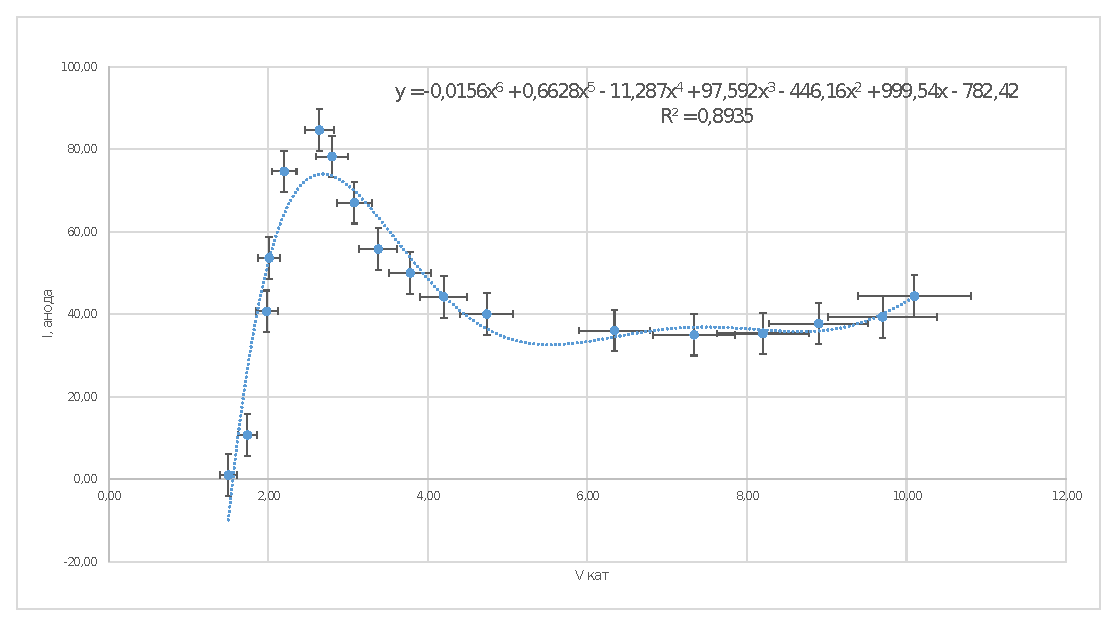
\includegraphics[width=\textwidth]{book1.eps}
    \end{floatrow}
    \caption{Зависимости вероятности рассеяния электронов от энергии}
\end{figure}
\end{document}